\section{Theoretical Analysis}
\label{Teorica}
\subsection{Gain Stage Description}

Firstly, we will make a brief description of how the gain stage works. As previously stated, its objective is to amplify the voltage input. In order to do so we utilize the following components: NPN BJT (negative-positive-negative bipolar junction transistor), Resistors, Capacitors and voltage sources.

The $V_{cc}$ voltage source is added with the objective of ensuring the transistor is acting in the Forward Active Region. The condition for operating in such region is $V_{CE}>V_{BE}$.

Both the capacitors have important functions within the circuit. The $C_{in}$ capacitor (coupling capacitor) acts as a DC block, ensuring that the transistor is in the desired operating region. The second capacitor, $C_E$, is a bypass capacitor. Taking a look at the formulae for the capacitor impedance: $\frac{1}{jwc}$, we can understand what this means. For low frequencies, the capacitor impedance is really high, which makes all the current flow through the RE resistor. On the other hand, for high frequencies, the capacitor impedance is really low, making it act almost as a short circuit. Therefore, almost all current flows through it.

It is also relevant to look at the impedance seen by the input voltage source, as it needs to be a lot greater than the resistance associated with the generator. The formulae is the following:

\begin{equation}
    Z_{I1}= (R_1 || R2) || r_{\pi 1}
\end{equation}


Taking a look at the output impedance formulae (\ref{form1}), we can see that it is really high, in comparison to the load resistance of 8 Ohm. Therefore, by the voltage divider rule, it becomes obvious that we need to add another stage to lower the impedance seen by the load. (note that we are doing a high-frequency analysis, considering $R_E \simeq 0$)

\begin{equation}
\label{form1}
     Z_{O1}=r_o || R_C
\end{equation}

\subsection{Output Stage Description}

As said before, the main goal of the output stage is to lower the output impedance.


For this stage, we utilized resistors, a capacitor, a PNP BJT and a voltage source.
Similarly to what was described in the previous stage, the voltage source is used to ensure the transistor operates in the desired region (forward active region), satisfying the condition for PNP BJT: $V_{EC}>V_{EB}$. Furthermore, the capacitor $C_O$ also acts as a coupling transistor, blocking the DC and ensuring the transistor stays in the forward active region.


Again, it is also relevant to look at the impedance seen by the input voltage source (\ref{form2}), as it needs to be much lower than $Z_{O1}$, so that there is no loss between both stages (voltage divider formulae, equation X). 

\begin{equation}
\label{form2}
    Z_{I2}=\frac{(g_{m2}+g_{\pi2}+g_{o2}+g_{E2})}{g_{\pi2}(g_{\pi2}+g_{o2}+g_{E2})}
\end{equation}

\begin{equation}
    V_{in2} = \frac{Z_{I2}}{Z_{I2}+Z_{O1}} V_{O2}. 
\end{equation}


Taking a look at the output impedance formulae (\ref{form3}), we that the output stage achieves its purpose of diminishing the impedance seen by the load.

\begin{equation}
\label{form3}
     Z_{O2}=\frac{1}{(g_{m2}+g_{\pi2}+g_{o2}+g_{E2})}
\end{equation}




\subsection{Merit Figure and Values Determination}

The main goal of this lab was to design the best possible audio amplification circuit. The quality of our work is evaluated with the calculation of a merit figure, which takes into account the following parameters:
-the voltage gain between the voltage generator input, and the load output; 
-the lower cut-off frequency (and higher cut-off frequency), which corresponds to the minimum (and maximum) frequency value of the bandwidth, and represents the first (and last) frequency for which the signal is correctly amplified, which is desired to be as low (as high) as possible. Both these frequencies are calculated by determining when the output voltage is 3db less than the gain;
-the bandwidth of our amplified signal, which is the range of frequencies for which our input signal is correctly amplified (it's calculated by subtracting the higher cut-off frequency by the lower cut-off frequency);
-the cost of the circuit.

The formulae for the merit figure is the following:


With the objective to obtain the biggest possible merit figure, we ran an optimization using Simulink, a very useful toolbox of the Matlab program. With this, we obtained the following values for our resistors and capacity of the capacitors:

\begin{table}[H]
\centering
\begin{tabularx}{0.6\textwidth} {
  | >{\raggedright\arraybackslash}X
  | >{\raggedleft\arraybackslash}X | }
 \hline
VCE & 6.698985e+00 V\\ \hline
VBEON & 7.000000e-01 V \\ \hline
VEC & 7.503512e+00 V\\ \hline
VEBON & 7.000000e-01 V \\ \hline
IB1 & 5.816344e-06 A \\ \hline
IC1 & 1.039381e-03 A \\ \hline
IE1 & 1.045197e-03 A \\ \hline
IB2 & -3.285189e-05 A \\ \hline
IC2 & 7.467235e-03 A \\ \hline
IE2 & 7.500087e-03 A \\ \hline
Merit & 4.922026e+02 \\ \hline
HighCutOff frequency & 4.378919e+05 Hz\\ \hline
LowCutOff frequency & 1.262636e+01 Hz\\ \hline
Cost & 2.198944e+03 MU's\\ \hline
Bandwidth & 4.378793e+05 Hz\\ \hline
Max Gain & 3.111592e+01 V\\ \hline

\end{tabularx}
\caption{Optimization results and merit}
\end{table}

After discovering all the needed values, we can also plot the gain, input and output impedances of both the circuits.

\begin{table}[H]
\centering
\begin{tabularx}{0.6\textwidth} {
  | >{\raggedright\arraybackslash}X
  | >{\raggedleft\arraybackslash}X | }
 \hline
AV1dB & 3.158539e+01 dB\\ \hline
ZI1 & 2.419648e+03 Omega \\ \hline
ZO1 & 4.652785e+03 Omega \\ \hline

\end{tabularx}
\caption{Gain stage: gain in dB, input and output impedance}
\end{table}

\begin{table}[H]
\centering
\begin{tabularx}{0.6\textwidth} {
  | >{\raggedright\arraybackslash}X
  | >{\raggedleft\arraybackslash}X | }
 \hline
AV2dB & -9.207782e-02 dB\\ \hline
ZI2 & 7.218471e+04 Omega \\ \hline
ZO2 & 3.313468e+00 Omega \\ \hline

\end{tabularx}
\caption{Output stage: gain in dB, input and output impedance}
\end{table}

\begin{table}[H]
\centering
\begin{tabularx}{0.6\textwidth} {
  | >{\raggedright\arraybackslash}X
  | >{\raggedleft\arraybackslash}X | }
 \hline
AVdB & 3.120876e+01 dB\\ \hline
ZO & 2.270796e+01 Omega\\ \hline

\end{tabularx}
\caption{Total circuit gain and output impedance}
\end{table}

And, finally, the frequency response $\frac{V_o(f)}{V_i(f)}$

\begin{figure}[H]\centering
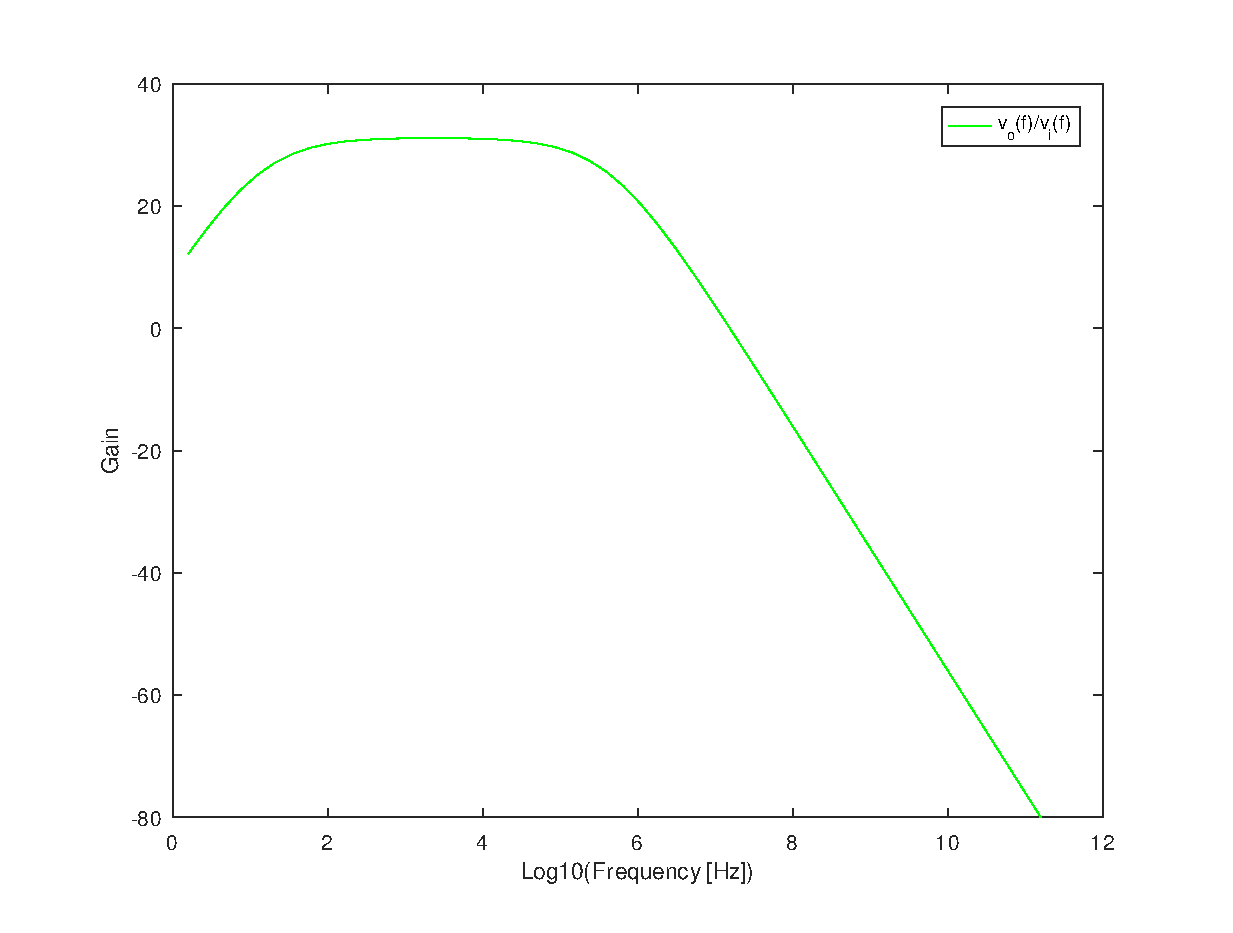
\includegraphics[width=0.7\linewidth]{grafico_octave.eps}
\caption{Octave Frequency response}
\label{fig:snat}
\end{figure}


